\documentclass{article}


% if you need to pass options to natbib, use, e.g.:
%     \PassOptionsToPackage{numbers, compress}{natbib}
% before loading neurips_2022


% ready for submission

\PassOptionsToPackage{square,sort,comma,numbers}{natbib}

\usepackage{neurips_2022}


% to compile a preprint version, e.g., for submission to arXiv, add add the
% [preprint] option:
%     \usepackage[preprint]{neurips_2022}


% to compile a camera-ready version, add the [final] option, e.g.:
%     \usepackage[final]{neurips_2022}


% to avoid loading the natbib package, add option nonatbib:
%    \usepackage[nonatbib]{neurips_2022}


\usepackage[utf8]{inputenc} % allow utf-8 input
\usepackage[T1]{fontenc}    % use 8-bit T1 fonts
\usepackage{hyperref}       % hyperlinks
\usepackage{url}            % simple URL typesetting
\usepackage{booktabs}       % professional-quality tables
\usepackage{amsfonts}       % blackboard math symbols
\usepackage{nicefrac}       % compact symbols for 1/2, etc.
\usepackage{microtype}      % microtypography
\usepackage{xcolor}         % colors
\usepackage{pgfplots}       % plots

\title{Comparative Study of Transformer-Based Large Language Models\\Final Report \\05/15/2023}


% The \author macro works with any number of authors. There are two commands
% used to separate the names and addresses of multiple authors: \And and \AND.
%
% Using \And between authors leaves it to LaTeX to determine where to break the
% lines. Using \AND forces a line break at that point. So, if LaTeX puts 3 of 4
% authors names on the first line, and the last on the second line, try using
% \AND instead of \And before the third author name.


\author{
  David S.~Hippocampus\thanks{Use footnote for providing further information
    about author (webpage, alternative address)---\emph{not} for acknowledging
    funding agencies.} \\
  Department of Computer Science\\
  Cranberry-Lemon University\\
  Pittsburgh, PA 15213 \\
  \texttt{hippo@cs.cranberry-lemon.edu} \\
  examples of more authors
  \And
  Man Liang \\
  University of Maryland \\
  Address \\
  \texttt{email} \\
  % \AND
  % Coauthor \\
  % Affiliation \\
  % Address \\
  % \texttt{email} \\
  % \And
  % Coauthor \\
  % Affiliation \\
  % Address \\
  % \texttt{email} \\
  % \And
  % Coauthor \\
  % Affiliation \\
  % Address \\
  % \texttt{email} \\
}


\begin{document}


\maketitle

\begin{abstract}
 This project proposal aims to review the spectrum of uses for Large Language Models, or LLMs, in Transformer models. Since LLMs have achieved great success in the past few years, including the recent ChatGPT model, it is interesting to see how different transformer-based models perform on different tasks, for example, Named Entity Recognition (NER), Natural Language Inference (NLI), and Question Answering (QA). 

 After a literature review process, this project will compare the performance of widely used transformer-based deep learning architectures on benchmark datasets in natural language processing. 
\end{abstract}


\section{Introduction}
Transformer-based models have become very popular in large language models and have achieved state-of-the-art performance on a variety of NLP tasks. The recent popular ChatGPT is a famous example. Transformer-based models were introduced in 2017 by Vaswani et al. The key innovation of them is the attention mechanism, which allows models to selectively focus on different parts of the input sequence while processing. Many transformer-based architectures are designed on various tasks, such as GPT, BERT, DistilBERT, XLNet, RoBERTa, etc. However, it is currently unknown how these models would perform on different tasks. It is a public perception that the GPT model is doing great in Question-Answering Tasks, but we don't know if or to what extent it will outperform the others. Motivated by this observation, we 
 set the research objective as understanding the performance of backbone architectures on common NLP tasks via literature survey and finetuning experiments. our research is designed with three major parts. First of all, we are going to conduct a literature survey of 5 widely used transformer-based architectures to get an overall understanding of these models and the current research trend. Second, we will finetune the models with benchmark datasets for three common NLP tasks: NER, NLI, and QA. Third, we will analyze and compare the performance of each model and its transferability. Our result would be compared with the findings from the literature survey to suggest the model selection. 

 \section{Literature Review}
 Recently, there have been substantial works to understand and improve transformer-based large language models. Clark, et al [1], studied the knowledge captured via the attention mechanisms of BERT. Hendrycks, et al [2] investigated out-of-distribution (OOD) generalization to improve model robustness. To get a holistic understanding of transformer-based models, several surveys were conducted. Kalyan, et al [3] and Min, et al [4] summarized the taxonomy and recent advances in this field. However, the survey was conducted at a high level in getting the big picture of the research field. No experiments were conducted to perform comparisons between different models for common NLP tasks. Therefore, there is a lack of literature to suggest model selection for solving practical problems.
 \subsection{Transformer Model}
 The transformer (Vaswani et al., 2017) model utilizes the attention mechanism as its core, in contrast to recurrent neural networks. The attention mechanism enables the model to focus on specific aspects of the text by learning the varying levels of importance of different text elements for a given task. For instance, words like "shopping" or "offer" may be highly relevant for filtering spam emails but not as important when analyzing sentiment. The attention mechanism determines this relevance by calculating a dynamically learned score for each element of the input sequence (value) and then computing the relative importance of the input sequence (key) for an output (query). Formally, attention maps a set of query, key, and value elements to an output, which is obtained by summing the weighted values, where the weights are determined by the compatibility (via dot product) between the query and the corresponding key.
 \subsection{Architectures}
\begin{itemize}
    \item BERT\\
    BERT (Bidirectional Encoder Representations from Transformers) is a transformer-based language model that uses a pre-training technique called Masked Language Modeling (MLM). BERT is primarily used for tasks such as question answering, text classification, and text similarity. 
    \item Distil-BERT \\
    Distil-BERT is a smaller and faster version of BERT that has been distilled to reduce its size and computational requirements. Despite the smaller size, Distil-BERT is still able to compete with BERT.
    \item XLNet \\
    XLNet is similar to other transformer-based models, such as BERT and RoBERTa, but it introduces several improvements that make it more powerful and flexible.
    \item RoBERTa \\
    RoBERTa (Robustly Optimized BERT pre-training approach) is a transformer-based language model that is similar to BERT but has been optimized for improved performance on various natural language processing tasks.
    \item ALBERT \\
    ALBERT (A Lite BERT) is a variant of the BERT (Bidirectional Encoder Representations from Transformers) model, which is a popular language representation model. ALBERT aims to reduce the computational resources required for training BERT by implementing parameter-sharing techniques, resulting in a smaller and more efficient model with comparable performance to BERT on various natural language processing tasks.
\end{itemize}
\subsection{Tasks and Benchmark Datasets}
As we delved into natural language processing (NLP) research, we examined several widely recognized benchmark datasets and their availability and reached the scope of our work below. 
\begin{itemize}
    \item NER \\
    Named Entity Recognition (NER) is a common task in NLP that involves identifying and classifying named entities in text, such as people, organizations, locations, and dates. The goal of NER is to automatically extract structured information from unstructured text. We are planning to use the WikiNEuRal EN dataset to perform model finetuning on NER.
        \begin{itemize}
            \item CoNLL-2003\\
            CoNLL-2003 is a popular dataset used in natural language processing (NLP) that contains labeled named entity recognition (NER) annotations for English language text, commonly used for training and evaluating NER models.
        \end{itemize}
    \item NLI \\
    Natural Language Inference (NLI) is another common task in NLP that determines the relationship between two text sequences. The goal is to infer and predict the relationship between a hypothesis and a given premise. We are planning to use the GLUE dataset for NLI task.
            \begin{itemize}
            \item GLUE\\
            GLUE benchmark dataset: A collection of diverse NLP tasks used for evaluating language models' performance and generalization in one sentence. It's also available on HuggingFace Datasets. We are focusing on the NLI tasks in GLUE for this project. 
        \end{itemize}
    \item QA \\
    Question answering (QA) is a task in natural language processing (NLP) that involves answering questions. It's aiming to provide a machine-readable answer to a human-generated question, given a large corpus of text as input. Recently released ChatGPT by OpenAI is an example. We will use SQuAD to finetune the architectures and evaluate them.
            \begin{itemize}
            \item SQuAD\\
            SQuAD is a question answering dataset that combines answerable questions from SQuAD1.1 with unanswerable questions designed to resemble answerable ones, challenging models to abstain from answering when no supported answer is available. It's accessible on HuggingFace Datasets.
        \end{itemize}
\end{itemize}
% \section{Methodology}

\section{Literature Survey}
\subsection{Survey Methods}
The literature survey acts as an important role to make our project successful. The objective of the literature survey is to get an overall understanding of the performance of the widely used transformer-based architectures in NLP tasks. In order to implement this approach, we conducted a literature review to identify papers that reported the performance of the 5 selected architectures on the benchmark dataset of interest. The result is summarized in the next section.

\subsection{Survey Result}

We have found the performance of target models on benchmark data from numerous different sources and have compiled the result into Table 1. In this table, we got the general sense that XLNet is good for NER, ALBERT is the best for both NLI and QA. 

\begin{table}[h]
    \centering
    \begin{tabular}{c|c|c|c|c}
        & NER(CoNLL 2003) & NLI(GLUE MNLI) & QA(SQuAD-1.1) &  \\
        & Accuracy & Matched & EM & F1\\
        \hline
        BERT finetune baseline & 92.4\%\ [5] & & 79.71 & 87.51 \\
        DistilBERT &  &  & 75.34 & 84.13 \\
        RoBERTa &  & 90.8\% & 85.42 & 91.82  \\
        XLNet & \textbf{93.28\%} [6] & & \textbf{89.898} & \textbf{95.080}  \\
        ALBERT &  & \textbf{91.3\%} & 82.69 & 90.25  \\
    \end{tabular}
    \caption{Summarize of Backbone Model on Benchmark Data}
    \label{tab:my_label}
\end{table}

From the literature survey, our observations are \\
\begin{itemize}
    \item Missing info for specific models on benchmark datasets within our consideration, which we'd like to experiment and fill in.
    \item All models tend to perform the best on NER, least on QA
    \item We don't know if there would be any model beat all in all tasks, which we will explore.
\end{itemize}

\section{Experiment Setup}
In this study, we are aiming to finetune 5 backbone transformer-based architectures on 3 selected tasks with benchmark datasets. We have replaced GPT architecture with ALBERT because limited literature was found for the former one. The other four architectures are BERT, Distil-BERT, XLNet, and RoBERTa. We are going to finetune the models according to the three common tasks, which are NER, NLI, and QA. A summary of our scope is in Table 2. For NER and NLI, we will use accuracy and F1 score to evaluate how good our models are and for QA, we will use EM(Exact Match) and F1 score. Accuracy is defined as the number of correct predictions divided by the total number of predictions. F1 score is another measure of accuracy. F1 score is calculated using the harmonic mean of precision and recall. This allows the F1 score to be a better measure of accuracy when there are class imbalances in the dataset. EM is an evaluation metric measuring the proportion of documents with the predicted answer being exactly the same as the correct answer.


\begin{table}[h]
    \centering
    \begin{tabular}{c|c|c}
       Tasks  & Benchmark Dataset & Evaluation Metrics \\
        NER & CoNll 2003 &Acc, F1 \\
        NLI & GLUE MNLI &Acc \\
        QA & SQuAD &EM, F1 \\
    \end{tabular}
    \caption{Task Scope}
    \label{tab:my_label}
\end{table}


\subsection{Code Setup and Test}
We have set up the basic codes for three selected tasks using the Transformer library with HuggingFace. To test the codes, we sampled a small subset from the benchmark datasets to make sure it works. The generic steps in the codes include:
\begin{itemize}
    \item import pre-trained model from HuggingFace Transformer library
    \item load benchmark datasets from HuggingFace Datasets library
    \item preprocessing the dataset: tokenization, padding, collation, etc.
    \item using HuggingFace Trainer API to train the model
    \item prepare the evaluation metrics
    \item evaluate and save the models
\end{itemize} A link to the codes is provided: \\
\textcolor{red}{https://github.com/censky2/CMSC742 }\\

As we are going to run 5 backbone models, we investigated and listed the pretrained models or model checkpoints below. As we planned, these pretrained model will be plugged into our code respectively and test, together with appropriate tokenizers and paddings.

\begin{itemize}
    \item BERT checkpoint: "bert-base-cased"
    \item DistilBert checkpoint: "distilbert-base-uncased"
    \item XLNet checkpoint: "xlnet-base-cased"
    \item RoBERTa checkpoint: "roberta-base"
    \item ALBERT checkpoint: "albert-base-v2"
\end{itemize}


\subsection{What we did}
\begin{itemize}
    \item Full Model Training \\
Our plan involves training a total of 15 tasks for each selected Language Model (LLM) model. This comprehensive training will include three different tasks for each individual model, resulting in a diverse and extensive training approach. We will start with the codes setup and replace with each backbone models. Given the magnitude of the task, we are considering the option of sampling a subset from the benchmark dataset, rather than training the entire set, in order to streamline the training process.
    \item Comparative Analysis \\
    From the model finetuning and evaluation section, we expected to get the performance of 5 pre-trained architectures and their finetuned version on 3 tasks. We are going to compare, analyze, and explain the performance of each backbone architecture and transferability. Our results would also be compared with the findings obtained from the literature survey section to capture similarities and differences. For example, GPT architecture is perceived as good at QA tasks, but our experiment result may suggest other architectures on a specific dataset.
\end{itemize}
% \subsubsection{Full Model Training}
% \section{Problem Setting}
% We are going to compare the performance of widely used transformer-based deep learning architectures on benchmark datasets in natural language processing. The performance and transferability of these models will be tested and evaluated on common NLP tasks including name entity recognition (NER), natural language inference (NLI), and question answering (QA). Additionally, we are going to compare the impact of both static embedding and contextualized embedding methods. Lastly, we will provide an analysis of the results. 
% \section{Methodology}
% In this study, we are going to complete three major tasks: literature survey, model finetuning, and comparative analysis. 

% \subsection{Model Finetuning}


% \subsubsection{Evaluation Metrics}
% % In the evaluation part, we are first going to report the generic performance of the finetuned models with different backbone architectures on each task planned. Typical metrics would include accuracy, precision, recall, F1 score or weighted F1 score. In addition, we'd like to learn the transferability ability of each backbone architecture on different tasks. Therefore, we would compare the performance of the finetuned model to the corresponding pre-trained model. Negative transfers may be observed. We would also try to quantify the transferability of the models, such as by adopting the LEEP score method.
% \subsubsection{Comparative Analysis}
\section{Results and Discussion}
\begin{table}[h]
    \centering
    \begin{tabular}{c|c|c|c|c|c}
        & NER(CoNLL 2003) & & NLI(GLUE MNLI) & QA(SQuAD) & \\
        & ACC & F1 & ACC & EM & F1 \\
        \hline
        BERT & 98.57\% & 94.44 \% & 82.42\%  & 78.70 & 86.67  \\
        DistilBERT & 98.58\% & 93.84\% & 80.68\%  & 72.89 & 82.24\\
        RoBERTa & 99.07\% & 95.93\% & \textbf{87.4\%} & 78.34 & 89.795 \\
        XLNet & \textbf{99.11\%} & \textbf{96.02\%} & 86.02\%  & 80.52 & 90.68 \\
        ALBERT & 98.46\% & 93.00\% & 83.5\% & \textbf{83.28} & \textbf{90.53} 
    \end{tabular}
    \caption{Experiment Results}
    \label{tab:my_label}
\end{table}
\begin{table}[h]
    \centering
    \begin{tabular}{c|c|c|c}
        & NER(CoNLL 2003) & NLI(GLUE MNLI) & QA(SQuAD) \\
        \hline
        Baseline & XLNet & ALBERT & XLNET  \\
        \hline
        Experiment & XLNet & XLNet & ALBERT  \\
    \end{tabular}
    \caption{Best Models}
    \label{tab:my_label}
\end{table}
The experimental results are presented in Table 3. Upon comparing the performance across three benchmark tasks, notable observations can be made. The NER (Named Entity Recognition) task exhibits exceptional accuracy, with all models achieving over 98\%. However, for the NLI (Natural Language Inference) task, accuracies range from 80\% to 88\%, while certain QA tasks experience a decline, with EM rates falling below 80\%. Intuitively, the task difficulty follows an ascending order of NER, NLI, and QA, which aligns with our findings and supports the observations documented in the literature survey.
Furthermore, Table 4 showcases our experiment results and provides distinct insights for model selection in the NLI and QA domains. We discovered that architectures with a higher number of hyperparameters tend to favor the NLI task. Conversely, the ALBERT architecture, which possesses a relatively lower number of hyperparameters, demonstrates greater benefits for the QA task. These findings highlight the importance of considering different architectural characteristics and hyperparameter configurations based on the specific task requirements.

\subsection{NER task observation}
\begin{figure}[h]
\centering
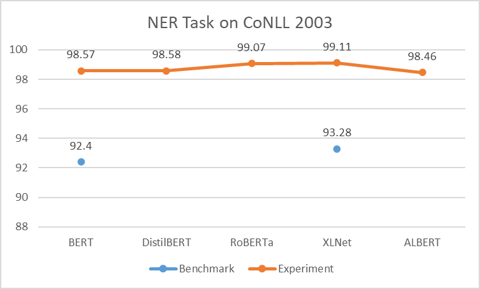
\includegraphics[width=0.8\columnwidth]{Picture4.png}
\caption{{NER Task: Accuracy comparative to baseline}}
\label{fig:lossimages}
\vspace{-1pt}
\end{figure}
The 5 models trained for the NER task were all trained using 10 epochs, a weight decay of 0.01 and learning rates of $2 \times 10^{-5}$. All 5 models performed better than the benchmarks as our models had accuracies around $97-98 \%$ whereas the benchmark accuracies were around $92\%$. However, it is important to note that those benchmarks were from 2018 and 2021. Current, more modern models are able to perform the NER task with accuracies up to $99\%$. \\
Additionally, BERT, DistilBERT, and RoBERTa were trained with the same parameters except for a varied learning rate of $2 \times 10^{-4}$. As expected, as learning rate decreased, the models tended to perform better. Interestingly, DistilBERT performed just as well as its nondistiled counterpart, BERT, despite having around 40\% less parameters.

\begin{table}[h]
    \centering
    \begin{tabular}{c|c|c|c|c}
        & Learning Rate = $2 \times 10^{-4}$ & & Learning Rate = $2 \times 10^{-5}$ &  \\
        & ACC & F1 & ACC & F1 \\
        \hline
        BERT & 97.54\%  & 89.73\% & 98.57\% & 94.44\% \\
        DistilBERT & 97.57\%  & 90.40\% & 98.58\% & 93.84\%\\
        RoBERTa & 98.11\% & 91.60\% & 99.07\% & 95.93\% \\
    \end{tabular}
    \caption{NER Experiment Results}
    \label{tab:my_label}
\end{table}
\begin{figure}[h]
\centering
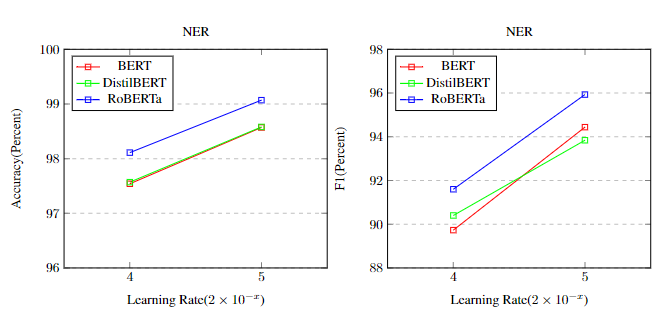
\includegraphics[width=1\columnwidth]{lr.png}
\caption{{NER task experiment results regarding learning rate}}
\label{fig:lossimages}
\vspace{-1pt}
\end{figure}


% \begin{tikzpicture}
% \begin{axis}[
%     title={NER},
%     xlabel={Learning Rate($2 \times 10^{-x}$)},
%     ylabel={Accuracy(Percent)},
%     xmin=3.5, xmax=5.5,
%     ymin=96, ymax=100,
%     xtick={4, 5},
%     ytick={96, 97, 98, 99, 100},
%     legend pos=north west,
%     ymajorgrids=true,
%     grid style=dashed,
% ]

% \addplot[
%     color=red,
%     mark=square,
%     ]
%     coordinates {
%     (4, 97.54)(5, 98.57)
%     };
%     \addlegendentry{BERT}

% \addplot[
%     color=green,
%     mark=square,
%     ]
%     coordinates {
%     (4, 97.57)(5, 98.58)
%     };
%     \addlegendentry{DistilBERT}

% \addplot[
%     color=blue,
%     mark=square,
%     ]
%     coordinates {
%     (4, 98.11)(5, 99.07)
%     };
%     \addlegendentry{RoBERTa}
    
% \end{axis}
% \end{tikzpicture}
% \begin{tikzpicture}
% \begin{axis}[
%     title={NER},
%     xlabel={Learning Rate($2 \times 10^{-x}$)},
%     ylabel={F1(Percent)},
%     xmin=3.5, xmax=5.5,
%     ymin=88, ymax=98,
%     xtick={4, 5},
%     ytick={88, 90, 92, 94, 96, 98},
%     legend pos=north west,
%     ymajorgrids=true,
%     grid style=dashed,
% ]

% \addplot[
%     color=red,
%     mark=square,
%     ]
%     coordinates {
%     (4, 89.73)(5, 94.44)
%     };
%     \addlegendentry{BERT}

% \addplot[
%     color=green,
%     mark=square,
%     ]
%     coordinates {
%     (4, 90.40)(5, 93.84)
%     };
%     \addlegendentry{DistilBERT}

% \addplot[
%     color=blue,
%     mark=square,
%     ]
%     coordinates {
%     (4, 91.60)(5, 95.93)
%     };
%     \addlegendentry{RoBERTa}
    
% \end{axis}
% \end{tikzpicture}


\subsection{NLI task observation}

\begin{figure}[h]
\centering
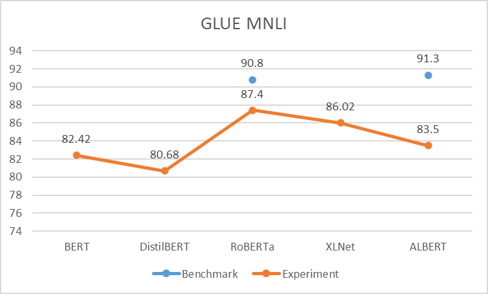
\includegraphics[width=0.8\columnwidth]{Picture2.png}
\caption{{NLI Task: Accuracy comparative to baseline}}
\label{fig:lossimages}
\vspace{-1pt}
\end{figure}

For the NLI task, we set the hyperparameters as the following: learning rate = $2 \times 10^{-5}$, number of epochs = 2, weight decay = 0.01. The comparative result over the baseline is provided in Figure 3. Surprisingly, our findings contradict the baseline results, where the ALBERT architecture performed the best. In our specific experiment, the RoBERTa model outperformed all others, with XLNet following closely behind. We speculate that this discrepancy arises from the substantial number of parameters in the RoBERTa model (125 million), which evidently provides significant advantages for the NLI task. Conversely, the embedding factorization and weight-sharing features inherent to the ALBERT architecture did not manifest effectively in our experiment. 




% \begin{figure}[H]
%     \centering
%     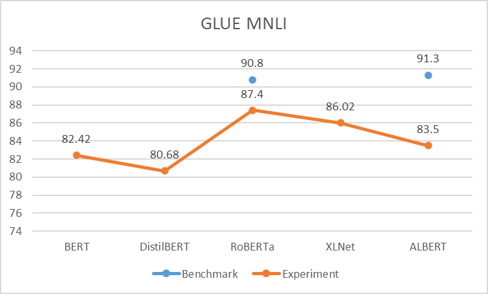
\includegraphics{Picture2.png}
%     \caption{Caption}
%     \label{fig:my_label}
% \end{figure}



\subsection{QA task observation}
\begin{figure}[h]
\centering
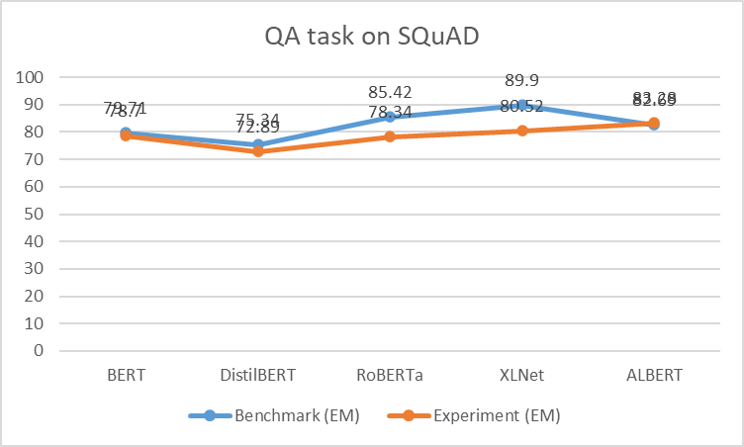
\includegraphics[width=0.8\columnwidth]{Picture3.png}
\caption{{QA task: Accuracy comparative to baseline}}
\label{fig:lossimages}
\vspace{-1pt}
\end{figure}
% \begin{figure}
%     \centering
%     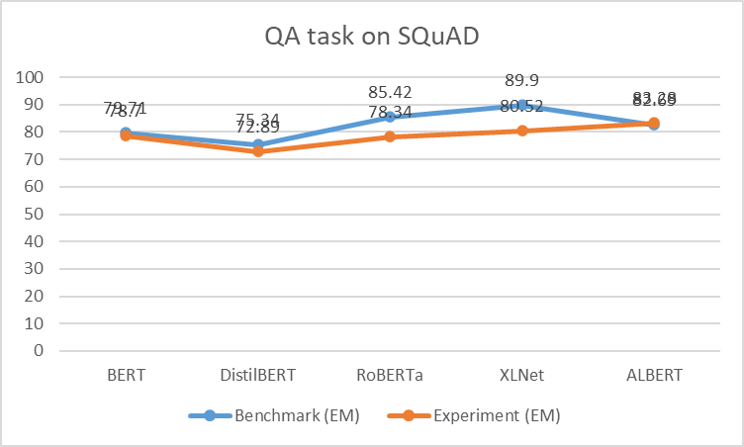
\includegraphics{Picture3.png}
%     \caption{Caption}
%     \label{fig:my_label}
% \end{figure}
The hyperparameters selected for the QA (Question Answering) task are as follows: learning rate = $2 \times 10^{-5}$, number of epochs = 1, weight decay = 0.01.  The comparative results are depicted in Figure 4, revealing that our experiment's performance closely aligns with the baselines, albeit with a slight underperformance. Notably, in our QA experiment on the SQuAD dataset, the ALBERT model emerges as the top-performing model, surpassing the baseline with an impressive exact match (EM) score of 83.28. Despite having only 12 million parameters, ALBERT's embedding factorization and weight sharing features proved to be advantageous for the QA task, a characteristic that was not as impactful in the NLI task. In contrast, we deduce that a greater number of hyperparameters tends to benefit NLI tasks, while the embedding factorization and weight sharing features are more advantageous for QA tasks.

\section{Conclusion}
In this project, we conducted a literature survey to understand transformer models architecture and performance and empirically finetuned 15 models on 5 architectures over 3 benchmark datasets. What we found was that the results differ from benchmark models and believe this provides us with new model selection insights. We found that, for model performance across 3 tasks over the benchmark datasets, the models performed NER the most accurately and QA the least. XLNet was also performed the best on NER and NLI and ALBERT performed the best on QA. We also found that our observed accuracies show differences compared to baselines and hypothesize that higher number of parameters favor NLI tasks whereas embedding factorization and weight sharing favor QA tasks, which is why ALBERT outperforms our XLNet at QA tasks 
 
\section{Future works}
It is important to acknowledge the limitations of our study. We must recognize that due to constraints in knowledge and computational resources at the time of conducting the work, we were unable to explore the complete landscape of hyperparameters and generate comprehensive results. Also, each of us is in charge of one task and the implementation details may be slightly different. which requires further validation of the results. We list the future works to improve our experiments as next steps. 
\begin{itemize}
    \item Investigate reasons for the gap between our results and the baseline
    \item Include other popular transformer models such as GPT-4
    \item Test and compare other hyper-params and metrics such as epochs, weight decays, to draw more general insights on model selection
    \item Employ ensemble learning to combine the models for each task
    \item Explore multi-task learning to train multi-head for all tasks
\end{itemize}

% \section{Challenges Until Now}
% \begin{itemize}
%     \item One of the challenges we faced was finding literature on the GPT model on the tasks we outlined. For that reason we decided not to commit to including GPT in our experiment setup. If we have time the resource left, we will add GPT model in and compare with the performance of the others.\\
%     \item We expect that we may need to train a minimum of 15 models (3x5), which could be excessive, so we will consider the possibility of sampling a subset of the benchmarks instead.

% \end{itemize}

% \begin{itemize}
%     \item Computational Resource: \\Training LLM requires extensive computational resources, especially the GPU. We are looking for resources besides the free offerings in Google CoLab. If constrained by resources, we may consider reducing the scope of pre-training models or sampling a portion of the datasets as this project progresses.
%     \item Model Selection: \\We selected five popular transformer-based LLM architectures to train. However, they may not be the best selections to make comparisons. Possible reasons could be that favored tasks for each model are not diversified, making the result hard to compare. We are doing literature surveys and looking for advice to refine the model selection strategy.
%     % \item Dataset Selection:
%     \item Team Competency: \\Our team was formed by students not currently enrolled as PhD students in computer science. We have limited knowledge of LLM and programming techniques. We treat this project as a learning journey to get the skills in studying and training transformer-based NLP models.
% \end{itemize}

% Please read the instructions below carefully and follow them faithfully.


% \subsection{Style}


% Papers to be submitted to NeurIPS 2022 must be prepared according to the
% instructions presented here. Papers may only be up to {\bf nine} pages long,
% including figures. Additional pages \emph{containing only acknowledgments and
% references} are allowed. Papers that exceed the page limit will not be
% reviewed, or in any other way considered for presentation at the conference.


% The margins in 2022 are the same as those in 2007, which allow for $\sim$$15\%$
% more words in the paper compared to earlier years.


% Authors are required to use the NeurIPS \LaTeX{} style files obtainable at the
% NeurIPS website as indicated below. Please make sure you use the current files
% and not previous versions. Tweaking the style files may be grounds for
% rejection.


% \subsection{Retrieval of style files}


% The style files for NeurIPS and other conference information are available on
% the World Wide Web at
% \begin{center}
%   \url{http://www.neurips.cc/}
% \end{center}
% The file \verb+neurips_2022.pdf+ contains these instructions and illustrates the
% various formatting requirements your NeurIPS paper must satisfy.


% The only supported style file for NeurIPS 2022 is \verb+neurips_2022.sty+,
% rewritten for \LaTeXe{}.  \textbf{Previous style files for \LaTeX{} 2.09,
%   Microsoft Word, and RTF are no longer supported!}


% The \LaTeX{} style file contains three optional arguments: \verb+final+, which
% creates a camera-ready copy, \verb+preprint+, which creates a preprint for
% submission to, e.g., arXiv, and \verb+nonatbib+, which will not load the
% \verb+natbib+ package for you in case of package clash.


% \paragraph{Preprint option}
% If you wish to post a preprint of your work online, e.g., on arXiv, using the
% NeurIPS style, please use the \verb+preprint+ option. This will create a
% nonanonymized version of your work with the text ``Preprint. Work in progress.''
% in the footer. This version may be distributed as you see fit. Please \textbf{do
%   not} use the \verb+final+ option, which should \textbf{only} be used for
% papers accepted to NeurIPS.


% At submission time, please omit the \verb+final+ and \verb+preprint+
% options. This will anonymize your submission and add line numbers to aid
% review. Please do \emph{not} refer to these line numbers in your paper as they
% will be removed during generation of camera-ready copies.


% The file \verb+neurips_2022.tex+ may be used as a ``shell'' for writing your
% paper. All you have to do is replace the author, title, abstract, and text of
% the paper with your own.


% The formatting instructions contained in these style files are summarized in
% Sections \ref{gen_inst}, \ref{headings}, and \ref{others} below.


% \section{General formatting instructions}
% \label{gen_inst}


% The text must be confined within a rectangle 5.5~inches (33~picas) wide and
% 9~inches (54~picas) long. The left margin is 1.5~inch (9~picas).  Use 10~point
% type with a vertical spacing (leading) of 11~points.  Times New Roman is the
% preferred typeface throughout, and will be selected for you by default.
% Paragraphs are separated by \nicefrac{1}{2}~line space (5.5 points), with no
% indentation.


% The paper title should be 17~point, initial caps/lower case, bold, centered
% between two horizontal rules. The top rule should be 4~points thick and the
% bottom rule should be 1~point thick. Allow \nicefrac{1}{4}~inch space above and
% below the title to rules. All pages should start at 1~inch (6~picas) from the
% top of the page.


% For the final version, authors' names are set in boldface, and each name is
% centered above the corresponding address. The lead author's name is to be listed
% first (left-most), and the co-authors' names (if different address) are set to
% follow. If there is only one co-author, list both author and co-author side by
% side.


% Please pay special attention to the instructions in Section \ref{others}
% regarding figures, tables, acknowledgments, and references.


% \section{Headings: first level}
% \label{headings}


% All headings should be lower case (except for first word and proper nouns),
% flush left, and bold.


% First-level headings should be in 12-point type.


% \subsection{Headings: second level}


% Second-level headings should be in 10-point type.


% \subsubsection{Headings: third level}


% Third-level headings should be in 10-point type.


% \paragraph{Paragraphs}


% There is also a \verb+\paragraph+ command available, which sets the heading in
% bold, flush left, and inline with the text, with the heading followed by 1\,em
% of space.


% \section{Citations, figures, tables, references}
% \label{others}


% These instructions apply to everyone.


% \subsection{Citations within the text}


% The \verb+natbib+ package will be loaded for you by default.  Citations may be
% author/year or numeric, as long as you maintain internal consistency.  As to the
% format of the references themselves, any style is acceptable as long as it is
% used consistently.


% The documentation for \verb+natbib+ may be found at
% \begin{center}
%   \url{http://mirrors.ctan.org/macros/latex/contrib/natbib/natnotes.pdf}
% \end{center}
% Of note is the command \verb+\citet+, which produces citations appropriate for
% use in inline text.  For example,
% \begin{verbatim}
%    \citet{hasselmo} investigated\dots
% \end{verbatim}
% produces
% \begin{quote}
%   Hasselmo, et al.\ (1995) investigated\dots
% \end{quote}


% If you wish to load the \verb+natbib+ package with options, you may add the
% following before loading the \verb+neurips_2022+ package:
% \begin{verbatim}
%    \PassOptionsToPackage{options}{natbib}
% \end{verbatim}


% If \verb+natbib+ clashes with another package you load, you can add the optional
% argument \verb+nonatbib+ when loading the style file:
% \begin{verbatim}
%    \usepackage[nonatbib]{neurips_2022}
% \end{verbatim}


% As submission is double blind, refer to your own published work in the third
% person. That is, use ``In the previous work of Jones et al.\ [4],'' not ``In our
% previous work [4].'' If you cite your other papers that are not widely available
% (e.g., a journal paper under review), use anonymous author names in the
% citation, e.g., an author of the form ``A.\ Anonymous.''


% \subsection{Footnotes}


% Footnotes should be used sparingly.  If you do require a footnote, indicate
% footnotes with a number\footnote{Sample of the first footnote.} in the
% text. Place the footnotes at the bottom of the page on which they appear.
% Precede the footnote with a horizontal rule of 2~inches (12~picas).


% Note that footnotes are properly typeset \emph{after} punctuation
% marks.\footnote{As in this example.}


% \subsection{Figures}


% \begin{figure}
%   \centering
%   \fbox{\rule[-.5cm]{0cm}{4cm} \rule[-.5cm]{4cm}{0cm}}
%   \caption{Sample figure caption.}
% \end{figure}


% All artwork must be neat, clean, and legible. Lines should be dark enough for
% purposes of reproduction. The figure number and caption always appear after the
% figure. Place one line space before the figure caption and one line space after
% the figure. The figure caption should be lower case (except for first word and
% proper nouns); figures are numbered consecutively.


% You may use color figures.  However, it is best for the figure captions and the
% paper body to be legible if the paper is printed in either black/white or in
% color.


% \subsection{Tables}


% All tables must be centered, neat, clean and legible.  The table number and
% title always appear before the table.  See Table~\ref{sample-table}.


% Place one line space before the table title, one line space after the
% table title, and one line space after the table. The table title must
% be lower case (except for first word and proper nouns); tables are
% numbered consecutively.


% Note that publication-quality tables \emph{do not contain vertical rules.} We
% strongly suggest the use of the \verb+booktabs+ package, which allows for
% typesetting high-quality, professional tables:
% \begin{center}
%   \url{https://www.ctan.org/pkg/booktabs}
% \end{center}
% This package was used to typeset Table~\ref{sample-table}.


% \begin{table}
%   \caption{Sample table title}
%   \label{sample-table}
%   \centering
%   \begin{tabular}{lll}
%     \toprule
%     \multicolumn{2}{c}{Part}                   \\
%     \cmidrule(r){1-2}
%     Name     & Description     & Size ($\mu$m) \\
%     \midrule
%     Dendrite & Input terminal  & $\sim$100     \\
%     Axon     & Output terminal & $\sim$10      \\
%     Soma     & Cell body       & up to $10^6$  \\
%     \bottomrule
%   \end{tabular}
% \end{table}


% \section{Final instructions}


% Do not change any aspects of the formatting parameters in the style files.  In
% particular, do not modify the width or length of the rectangle the text should
% fit into, and do not change font sizes (except perhaps in the
% \textbf{References} section; see below). Please note that pages should be
% numbered.


% \section{Preparing PDF files}


% Please prepare submission files with paper size ``US Letter,'' and not, for
% example, ``A4.''


% Fonts were the main cause of problems in the past years. Your PDF file must only
% contain Type 1 or Embedded TrueType fonts. Here are a few instructions to
% achieve this.


% \begin{itemize}


% \item You should directly generate PDF files using \verb+pdflatex+.


% \item You can check which fonts a PDF files uses.  In Acrobat Reader, select the
%   menu Files$>$Document Properties$>$Fonts and select Show All Fonts. You can
%   also use the program \verb+pdffonts+ which comes with \verb+xpdf+ and is
%   available out-of-the-box on most Linux machines.


% \item The IEEE has recommendations for generating PDF files whose fonts are also
%   acceptable for NeurIPS. Please see
%   \url{http://www.emfield.org/icuwb2010/downloads/IEEE-PDF-SpecV32.pdf}


% \item \verb+xfig+ "patterned" shapes are implemented with bitmap fonts.  Use
%   "solid" shapes instead.


% \item The \verb+\bbold+ package almost always uses bitmap fonts.  You should use
%   the equivalent AMS Fonts:
% \begin{verbatim}
%    \usepackage{amsfonts}
% \end{verbatim}
% followed by, e.g., \verb+\mathbb{R}+, \verb+\mathbb{N}+, or \verb+\mathbb{C}+
% for $\mathbb{R}$, $\mathbb{N}$ or $\mathbb{C}$.  You can also use the following
% workaround for reals, natural and complex:
% \begin{verbatim}
%    \newcommand{\RR}{I\!\!R} %real numbers
%    \newcommand{\Nat}{I\!\!N} %natural numbers
%    \newcommand{\CC}{I\!\!\!\!C} %complex numbers
% \end{verbatim}
% Note that \verb+amsfonts+ is automatically loaded by the \verb+amssymb+ package.


% \end{itemize}


% If your file contains type 3 fonts or non embedded TrueType fonts, we will ask
% you to fix it.


% \subsection{Margins in \LaTeX{}}


% Most of the margin problems come from figures positioned by hand using
% \verb+\special+ or other commands. We suggest using the command
% \verb+\includegraphics+ from the \verb+graphicx+ package. Always specify the
% figure width as a multiple of the line width as in the example below:
% \begin{verbatim}
%    \usepackage[pdftex]{graphicx} ...
%    \includegraphics[width=0.8\linewidth]{myfile.pdf}
% \end{verbatim}
% See Section 4.4 in the graphics bundle documentation
% (\url{http://mirrors.ctan.org/macros/latex/required/graphics/grfguide.pdf})


% A number of width problems arise when \LaTeX{} cannot properly hyphenate a
% line. Please give LaTeX hyphenation hints using the \verb+\-+ command when
% necessary.


% \begin{ack}
% Use unnumbered first level headings for the acknowledgments. All acknowledgments
% go at the end of the paper before the list of references. Moreover, you are required to declare
% funding (financial activities supporting the submitted work) and competing interests (related financial activities outside the submitted work).
% More information about this disclosure can be found at: \url{https://neurips.cc/Conferences/2022/PaperInformation/FundingDisclosure}.


% Do {\bf not} include this section in the anonymized submission, only in the final paper. You can use the \texttt{ack} environment provided in the style file to autmoatically hide this section in the anonymized submission.
% \end{ack}


% \section*{References}

\begin{thebibliography}{100} % 100 is a random guess of the total number of
%references
    \bibitem{1} Clark, K., Khandelwal, U., Levy, O. and Manning, C.D., 2019. What does bert look at? an analysis of bert's attention. arXiv preprint arXiv:1906.04341.
    \bibitem{2} Hendrycks, D., Liu, X., Wallace, E., Dziedzic, A., Krishnan, R. and Song, D., 2020. Pretrained transformers improve out-of-distribution robustness. arXiv preprint arXiv:2004.06100.
    \bibitem{3} Kalyan, K.S., Rajasekharan, A. and Sangeetha, S., 2021. Ammus: A survey of transformer-based pretrained models in natural language processing. arXiv preprint arXiv:2108.05542.
    \bibitem{4} Min, B., Ross, H., Sulem, E., Veyseh, A.P.B., Nguyen, T.H., Sainz, O., Agirre, E., Heinz, I. and Roth, D., 2021. Recent advances in natural language processing via large pre-trained language models: A survey. arXiv preprint arXiv:2111.01243.
\bibitem{DBLP:journals/corr/abs-1810-04805}
Jacob Devlin, Ming{-}Wei Chang, Kenton Lee, and Kristina Toutanova.
\newblock {BERT:} Pre-training of Deep Bidirectional Transformers for Language Understanding.
\newblock {\em CoRR}, volume abs/1810.04805, 2018.
\newblock URL: \url{http://arxiv.org/abs/1810.04805}.
\bibitem{DBLP:journals/corr/abs-2112-08033}
Tran Thi Hong Hanh, Antoine Doucet, Nicolas Sidere, Jos{\'{e}} G. Moreno, and Senja Pollak.
\newblock Named entity recognition architecture combining contextual and global features.
\newblock {\em CoRR}, volume abs/2112.08033, 2021.
\newblock URL: \url{https://arxiv.org/abs/2112.08033}.

\bibitem{DBLP:journals/corr/abs-1910-01108}
Victor Sanh, Lysandre Debut, Julien Chaumond, and Thomas Wolf.
\newblock DistilBERT, a distilled version of {BERT:} smaller, faster, cheaper and lighter.
\newblock {\em CoRR}, volume abs/1910.01108, 2019.
\newblock URL: \url{http://arxiv.org/abs/1910.01108}.
\newblock eprinttype = {arXiv}, eprint = {1910.01108}, timestamp = {Tue, 02 Jun 2020 12:48:59 +0200}.
\newblock BibURL: \url{https://dblp.org/rec/journals/corr/abs-1910-01108.bib}.
\newblock BibSource: dblp computer science bibliography, \url{https://dblp.org}.


    
\end{thebibliography}

\bibliography{citation} 
% References follow the acknowledgments. Use unnumbered first-level heading for
% the references. Any choice of citation style is acceptable as long as you are
% consistent. It is permissible to reduce the font size to \verb+small+ (9 point)
% when listing the references.
% Note that the Reference section does not count towards the page limit.
% \medskip


% {
% \small


% [1] Alexander, J.A.\ \& Mozer, M.C.\ (1995) Template-based algorithms for
% connectionist rule extraction. In G.\ Tesauro, D.S.\ Touretzky and T.K.\ Leen
% (eds.), {\it Advances in Neural Information Processing Systems 7},
% pp.\ 609--616. Cambridge, MA: MIT Press.


% [2] Bower, J.M.\ \& Beeman, D.\ (1995) {\it The Book of GENESIS: Exploring
%   Realistic Neural Models with the GEneral NEural SImulation System.}  New York:
% TELOS/Springer--Verlag.


% [3] Hasselmo, M.E., Schnell, E.\ \& Barkai, E.\ (1995) Dynamics of learning and
% recall at excitatory recurrent synapses and cholinergic modulation in rat
% hippocampal region CA3. {\it Journal of Neuroscience} {\bf 15}(7):5249-5262.
% }


% %%%%%%%%%%%%%%%%%%%%%%%%%%%%%%%%%%%%%%%%%%%%%%%%%%%%%%%%%%%%
% \section*{Checklist}


% %%% BEGIN INSTRUCTIONS %%%
% The checklist follows the references.  Please
% read the checklist guidelines carefully for information on how to answer these
% questions.  For each question, change the default \answerTODO{} to \answerYes{},
% \answerNo{}, or \answerNA{}.  You are strongly encouraged to include a {\bf
% justification to your answer}, either by referencing the appropriate section of
% your paper or providing a brief inline description.  For example:
% \begin{itemize}
%   \item Did you include the license to the code and datasets? \answerYes{See Section~\ref{gen_inst}.}
%   \item Did you include the license to the code and datasets? \answerNo{The code and the data are proprietary.}
%   \item Did you include the license to the code and datasets? \answerNA{}
% \end{itemize}
% Please do not modify the questions and only use the provided macros for your
% answers.  Note that the Checklist section does not count towards the page
% limit.  In your paper, please delete this instructions block and only keep the
% Checklist section heading above along with the questions/answers below.
% %%% END INSTRUCTIONS %%%


% \begin{enumerate}


% \item For all authors...
% \begin{enumerate}
%   \item Do the main claims made in the abstract and introduction accurately reflect the paper's contributions and scope?
%     \answerTODO{}
%   \item Did you describe the limitations of your work?
%     \answerTODO{}
%   \item Did you discuss any potential negative societal impacts of your work?
%     \answerTODO{}
%   \item Have you read the ethics review guidelines and ensured that your paper conforms to them?
%     \answerTODO{}
% \end{enumerate}


% \item If you are including theoretical results...
% \begin{enumerate}
%   \item Did you state the full set of assumptions of all theoretical results?
%     \answerTODO{}
%         \item Did you include complete proofs of all theoretical results?
%     \answerTODO{}
% \end{enumerate}


% \item If you ran experiments...
% \begin{enumerate}
%   \item Did you include the code, data, and instructions needed to reproduce the main experimental results (either in the supplemental material or as a URL)?
%     \answerTODO{}
%   \item Did you specify all the training details (e.g., data splits, hyperparameters, how they were chosen)?
%     \answerTODO{}
%         \item Did you report error bars (e.g., with respect to the random seed after running experiments multiple times)?
%     \answerTODO{}
%         \item Did you include the total amount of compute and the type of resources used (e.g., type of GPUs, internal cluster, or cloud provider)?
%     \answerTODO{}
% \end{enumerate}


% \item If you are using existing assets (e.g., code, data, models) or curating/releasing new assets...
% \begin{enumerate}
%   \item If your work uses existing assets, did you cite the creators?
%     \answerTODO{}
%   \item Did you mention the license of the assets?
%     \answerTODO{}
%   \item Did you include any new assets either in the supplemental material or as a URL?
%     \answerTODO{}
%   \item Did you discuss whether and how consent was obtained from people whose data you're using/curating?
%     \answerTODO{}
%   \item Did you discuss whether the data you are using/curating contains personally identifiable information or offensive content?
%     \answerTODO{}
% \end{enumerate}


% \item If you used crowdsourcing or conducted research with human subjects...
% \begin{enumerate}
%   \item Did you include the full text of instructions given to participants and screenshots, if applicable?
%     \answerTODO{}
%   \item Did you describe any potential participant risks, with links to Institutional Review Board (IRB) approvals, if applicable?
%     \answerTODO{}
%   \item Did you include the estimated hourly wage paid to participants and the total amount spent on participant compensation?
%     \answerTODO{}
% \end{enumerate}


% \end{enumerate}


% %%%%%%%%%%%%%%%%%%%%%%%%%%%%%%%%%%%%%%%%%%%%%%%%%%%%%%%%%%%%


% \appendix


% \section{Appendix}


% Optionally include extra information (complete proofs, additional experiments and plots) in the appendix.
% This section will often be part of the supplemental material.


\end{document}
